\documentclass[12pt, oneside, letterpaper]{book}
\usepackage{configuraciones/setup}

% Casos de USO
% ==============================================================================
% LIBRERÍA DE DIAGRAMAS TIKZ - VERSIÓN CORREGIDA (SIN ENCIMAMIENTOS)
% ==============================================================================

\tikzset{
    actor/.style={thick},
    sistema/.style={thick, fill=gray!5},
    caso/.style={draw, ellipse, fill=azulESCOM!15, minimum width=4.5cm, minimum height=0.8cm, align=center},
    relación/.style={thick},
    extension/.style={thick, dashed, <-, >=stealth}
}

\newcommand{\dibujarQuejoso}[2]{
    \draw[actor] (#1,#2+0.7) circle (0.2); 
    \draw[actor] (#1,#2+0.5) -- (#1,#2); 
    \draw[actor] (#1-0.3,0.3+#2) -- (#1+0.3,0.3+#2); 
    \draw[actor] (#1,#2) -- (#1-0.2,#2-0.3); 
    \draw[actor] (#1,#2) -- (#1+0.2,#2-0.3); 
    \node at (#1,#2-0.6) {\scriptsize Quejoso};
}

% --- FIGURAS CORREGIDAS ---

% MODULO PERFIL
\newcommand{\figCUuno}{ \begin{tikzpicture}[font=\small] \dibujarQuejoso{-4}{2} \draw[sistema] (-1.5,0.5) rectangle (6,3.5); \node[anchor=north] at (2.25,3.4) {\textbf{\scriptsize Gestión de Perfil}}; \node[caso] (c) at (2.25,2) {\scriptsize CU01: Crear cuenta de usuario}; \draw[relación] (-3.7,2.3) -- (c.west); \end{tikzpicture} }

\newcommand{\figCUdos}{ \begin{tikzpicture}[font=\small] \dibujarQuejoso{-4}{2} \draw[sistema] (-1.5,0.5) rectangle (6,3.5); \node[anchor=north] at (2.25,3.4) {\textbf{\scriptsize Gestión de Perfil}}; \node[caso] (c) at (2.25,2) {\scriptsize CU02: Iniciar sesión}; \draw[relación] (-3.7,2.3) -- (c.west); \end{tikzpicture} }

\newcommand{\figCUtres}{ \begin{tikzpicture}[font=\small] \dibujarQuejoso{-4}{2.5} \draw[sistema] (-1.5,-0.5) rectangle (6,5); \node[caso] (c2) at (2.25,4) {\scriptsize CU02: Iniciar sesión}; \node[caso] (c3) at (2.25,0.5) {\scriptsize CU03: Recuperar contraseña}; \draw[extension] (c2) -- (c3) node[midway, right=0.2cm] {\tiny $<<Extend>>$}; \draw[relación] (-3.7,2.8) -- (c2.west); \end{tikzpicture} }

\newcommand{\figCUcuatro}{ \begin{tikzpicture}[font=\small] \dibujarQuejoso{-4}{2} \draw[sistema] (-1.5,0.5) rectangle (6,3.5); \node[caso] (c) at (2.25,2) {\scriptsize CU04: Editar perfil de usuario}; \draw[relación] (-3.7,2.3) -- (c.west); \end{tikzpicture} }

\newcommand{\figCUcinco}{ \begin{tikzpicture}[font=\small] \dibujarQuejoso{-4}{2} \draw[sistema] (-1.5,0.5) rectangle (6,3.5); \node[caso] (c) at (2.25,2) {\scriptsize CU05: Registrar datos de tutor}; \draw[relación] (-3.7,2.3) -- (c.west); \end{tikzpicture} }

% MODULO QUEJAS
\newcommand{\figCUseis}{ \begin{tikzpicture}[font=\small] \dibujarQuejoso{-4}{2} \draw[sistema] (-1.5,0.5) rectangle (6,3.5); \node[caso] (c) at (2.25,2) {\scriptsize CU06: Levantar queja}; \draw[relación] (-3.7,2.3) -- (c.west); \end{tikzpicture} }

\newcommand{\figCUsiete}{ \begin{tikzpicture}[font=\small] \dibujarQuejoso{-4}{2} \draw[sistema] (-1.5,0.5) rectangle (6,3.5); \node[caso] (c) at (2.25,2) {\scriptsize CU07: Adjuntar evidencia}; \draw[relación] (-3.7,2.3) -- (c.west); \end{tikzpicture} }

\newcommand{\figCUocho}{ \begin{tikzpicture}[font=\small] \dibujarQuejoso{-4}{2} \draw[sistema] (-1.5,0.5) rectangle (6,3.5); \node[caso] (c) at (2.25,2) {\scriptsize CU08: Consultar tablero de trámites}; \draw[relación] (-3.7,2.3) -- (c.west); \end{tikzpicture} }

% FIGURAS CON EXTENDS (CORREGIDAS)
\newcommand{\figCUnueve}{ \begin{tikzpicture}[font=\small] \dibujarQuejoso{-4}{2} \node[caso] (c6) at (0,2) {\scriptsize CU06: Levantar queja}; \node[caso] (c9) at (6,2) {\scriptsize CU09: Modificar queja}; \draw[extension] (c6) -- (c9) node[midway, above=0.1cm] {\tiny $<<Extend>>$}; \draw[relación] (-3.7,2.3) -- (c6.west); \end{tikzpicture} }

\newcommand{\figCUdiez}{ \begin{tikzpicture}[font=\small] \dibujarQuejoso{-4}{2} \node[caso] (c6) at (0,2) {\scriptsize CU06: Levantar queja}; \node[caso] (c10) at (6,2) {\scriptsize CU10: Eliminar borrador}; \draw[extension] (c6) -- (c10) node[midway, above=0.1cm] {\tiny $<<Extend>>$}; \draw[relación] (-3.7,2.3) -- (c6.west); \end{tikzpicture} }

\newcommand{\figCUonce}{ \begin{tikzpicture}[font=\small] \dibujarQuejoso{-4}{2} \draw[sistema] (-1.5,0.5) rectangle (6,3.5); \node[caso] (c) at (2.25,2) {\scriptsize CU11: Recibir notificaciones}; \draw[relación] (-3.7,2.3) -- (c.west); \end{tikzpicture} }

\newcommand{\figCUdoce}{ \begin{tikzpicture}[font=\small] \dibujarQuejoso{-4}{2} \node[caso] (c11) at (0,2) {\scriptsize CU11: Notificaciones}; \node[caso] (c12) at (6,2) {\scriptsize CU12: Completar información}; \draw[extension] (c11) -- (c12) node[midway, above=0.1cm] {\tiny $<<Extend>>$}; \draw[relación] (-3.7,2.3) -- (c11.west); \end{tikzpicture} }

\newcommand{\figCUtrece}{ \begin{tikzpicture}[font=\small] \dibujarQuejoso{-4}{2} \node[caso] (c11) at (0,2) {\scriptsize CU11: Notificaciones}; \node[caso] (c13) at (6,2) {\scriptsize CU13: Medidas precautorias}; \draw[extension] (c11) -- (c13) node[midway, above=0.1cm] {\tiny $<<Extend>>$}; \draw[relación] (-3.7,2.3) -- (c11.west); \end{tikzpicture} }

\newcommand{\figCUcatorce}{ \begin{tikzpicture}[font=\small] \dibujarQuejoso{-4}{2} \node[caso] (c11) at (0,2) {\scriptsize CU11: Notificaciones}; \node[caso] (c14) at (6,2) {\scriptsize CU14: Propuesta conciliación}; \draw[extension] (c11) -- (c14) node[midway, above=0.1cm] {\tiny $<<Extend>>$}; \draw[relación] (-3.7,2.3) -- (c11.west); \end{tikzpicture} }

\newcommand{\figCUquince}{ \begin{tikzpicture}[font=\small] \dibujarQuejoso{-4}{2} \node[caso] (c14) at (0,2) {\scriptsize CU14: Propuesta}; \node[caso] (c15) at (6,2) {\scriptsize CU15: Aceptar propuesta}; \draw[extension] (c14) -- (c15) node[midway, above=0.1cm] {\tiny $<<Extend>>$}; \draw[relación] (-3.7,2.3) -- (c14.west); \end{tikzpicture} }

\newcommand{\figCUdieciseis}{ \begin{tikzpicture}[font=\small] \dibujarQuejoso{-4}{2} \node[caso] (c14) at (0,2) {\scriptsize CU14: Propuesta}; \node[caso] (c16) at (6,2) {\scriptsize CU16: Rechazar propuesta}; \draw[extension] (c14) -- (c16) node[midway, above=0.1cm] {\tiny $<<Extend>>$}; \draw[relación] (-3.7,2.3) -- (c14.west); \end{tikzpicture} }

\newcommand{\figCUdiecisiete}{ \begin{tikzpicture}[font=\small] \dibujarQuejoso{-4}{2} \draw[sistema] (-1.5,0.5) rectangle (6,3.5); \node[caso] (c) at (2.25,2) {\scriptsize CU17: Descargar acuse}; \draw[relación] (-3.7,2.3) -- (c.west); \end{tikzpicture} }

\newcommand{\figCUdieciocho}{ \begin{tikzpicture}[font=\small] \dibujarQuejoso{-4}{2} \draw[sistema] (-1.5,0.5) rectangle (6,3.5); \node[caso] (c) at (2.25,2) {\scriptsize CU18: Detalles completos}; \draw[relación] (-3.7,2.3) -- (c.west); \end{tikzpicture} }
\usepackage[utf8]{inputenc}
\usepackage{textcomp}
\lstset{inputencoding=utf8, extendedchars=true}

% Imágenes y PDFs
\usepackage{pdfpages}
\usepackage{ragged2e}

% Definición de estilo para JSON
\lstdefinelanguage{json}{
    basicstyle=\normalfont\ttfamily\small,
    numbers=left,
    numberstyle=\scriptsize,
    stepnumber=1,
    numbersep=8pt,
    showstringspaces=false,
    breaklines=true,
    frame=lines,
    backgroundcolor=\color{gray!5}
}

\usepackage{tabularx}
\usepackage{enumitem}
\usepackage[table]{xcolor}

% ==============================================================================
\usepackage{hyperref}
\hypersetup{
    colorlinks=true,
    linkcolor=blue,
    urlcolor=blue,
    pdftitle={Trabajo Terminal - Defensoría de los Derechos Politécnicos},
    pdfnewwindow=true
}

\begin{document}

\section{Diagrama de Actividades}

El presente anexo concentra los diagramas de actividades correspondientes a los distintos departamentos de la DDP que conforman el sistema en general. Su propósito es representar, mediante notación UML, el flujo de trabajo de cada perfil dentro del sistema, mostrando las acciones y decisiones que componen los procesos operativos. 

Los diagramas se organizan por departamento (Quejoso, Recepción, Primer Contacto, Subdefensoría, Defensoría y Administración de TI) con el fin de ofrecer una visión integral del comportamiento del sistema y facilitar la comprensión de las responsabilidades asignadas a cada actor a lo largo del ciclo de atención de una queja.

\subsection{Microservicio: Quejoso}
\label{sec:da_quejoso}

El diagrama de actividades presentado en esta sección describe el flujo general de trabajo del perfil Quejoso dentro de la plataforma. 

Debido a la extensión del diagrama completo, este se ha dividido en dos partes para facilitar su lectura: la primera parte abarca el flujo desde el acceso inicial al portal hasta el levantamiento de la queja, mientras que la segunda parte continúa con las actividades posteriores relacionadas con la autenticación y entrada al dashboard del usuario, mostrando las acciones de consulta, modificación y seguimiento de quejas.

    % ---- DA-Quejoso Parte 1 ----
    \subsubsection{Diagrama de Actividades del Quejoso (Parte 1)}

    Primera parte del diagrama de actividades general del Quejoso. Representa las actividades iniciales del usuario en la plataforma: el acceso al portal, las decisiones entre registrar una nueva queja o dar seguimiento a un trámite existente sin iniciar sesión y el flujo de captura de información de la queja.
    \begin{figure}[H]
        \centering
        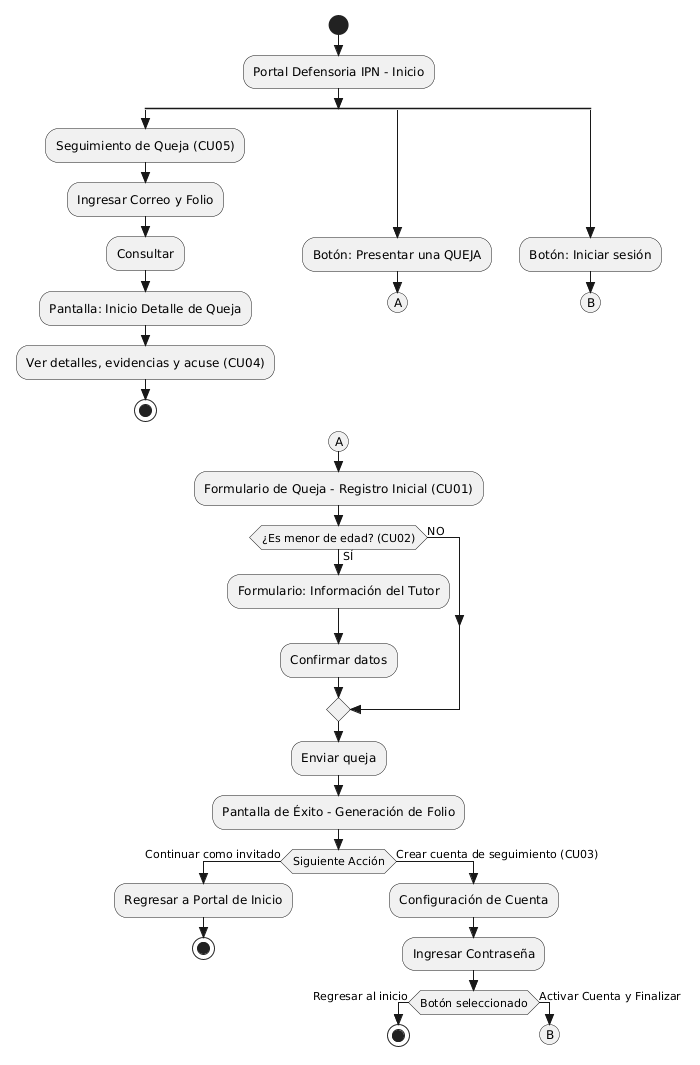
\includegraphics[width=0.90\textwidth, height=0.85\textheight, keepaspectratio]{imagenes/quejoso/D_Actividad/P1_DA-Quejoso.png}
        \caption{Diagrama de Actividades del Quejoso - Parte 1}
        \label{fig:da_quejoso_parte1}
    \end{figure}

    \clearpage

    % ---- DA-Quejoso Parte 2 ----
    \subsubsection{Diagrama de Actividades del Quejoso (Parte 2)}

    La segunda parte del diagrama de actividades general del Quejoso continúa el flujo en las rutas de autenticación y creación de cuenta para el seguimiento del expediente.
   Una vez que el usuario inicia sesion, entra en el dashboard, mostrando las actividades de consulta, modificación y eliminación de quejas, levantamiento de quejas, la revisión de notificaciones y el proceso de respuesta ante propuestas de conciliación emitidas por la Defensoría, hasta la finalización del trámite.

    \begin{figure}[H]
        \centering
        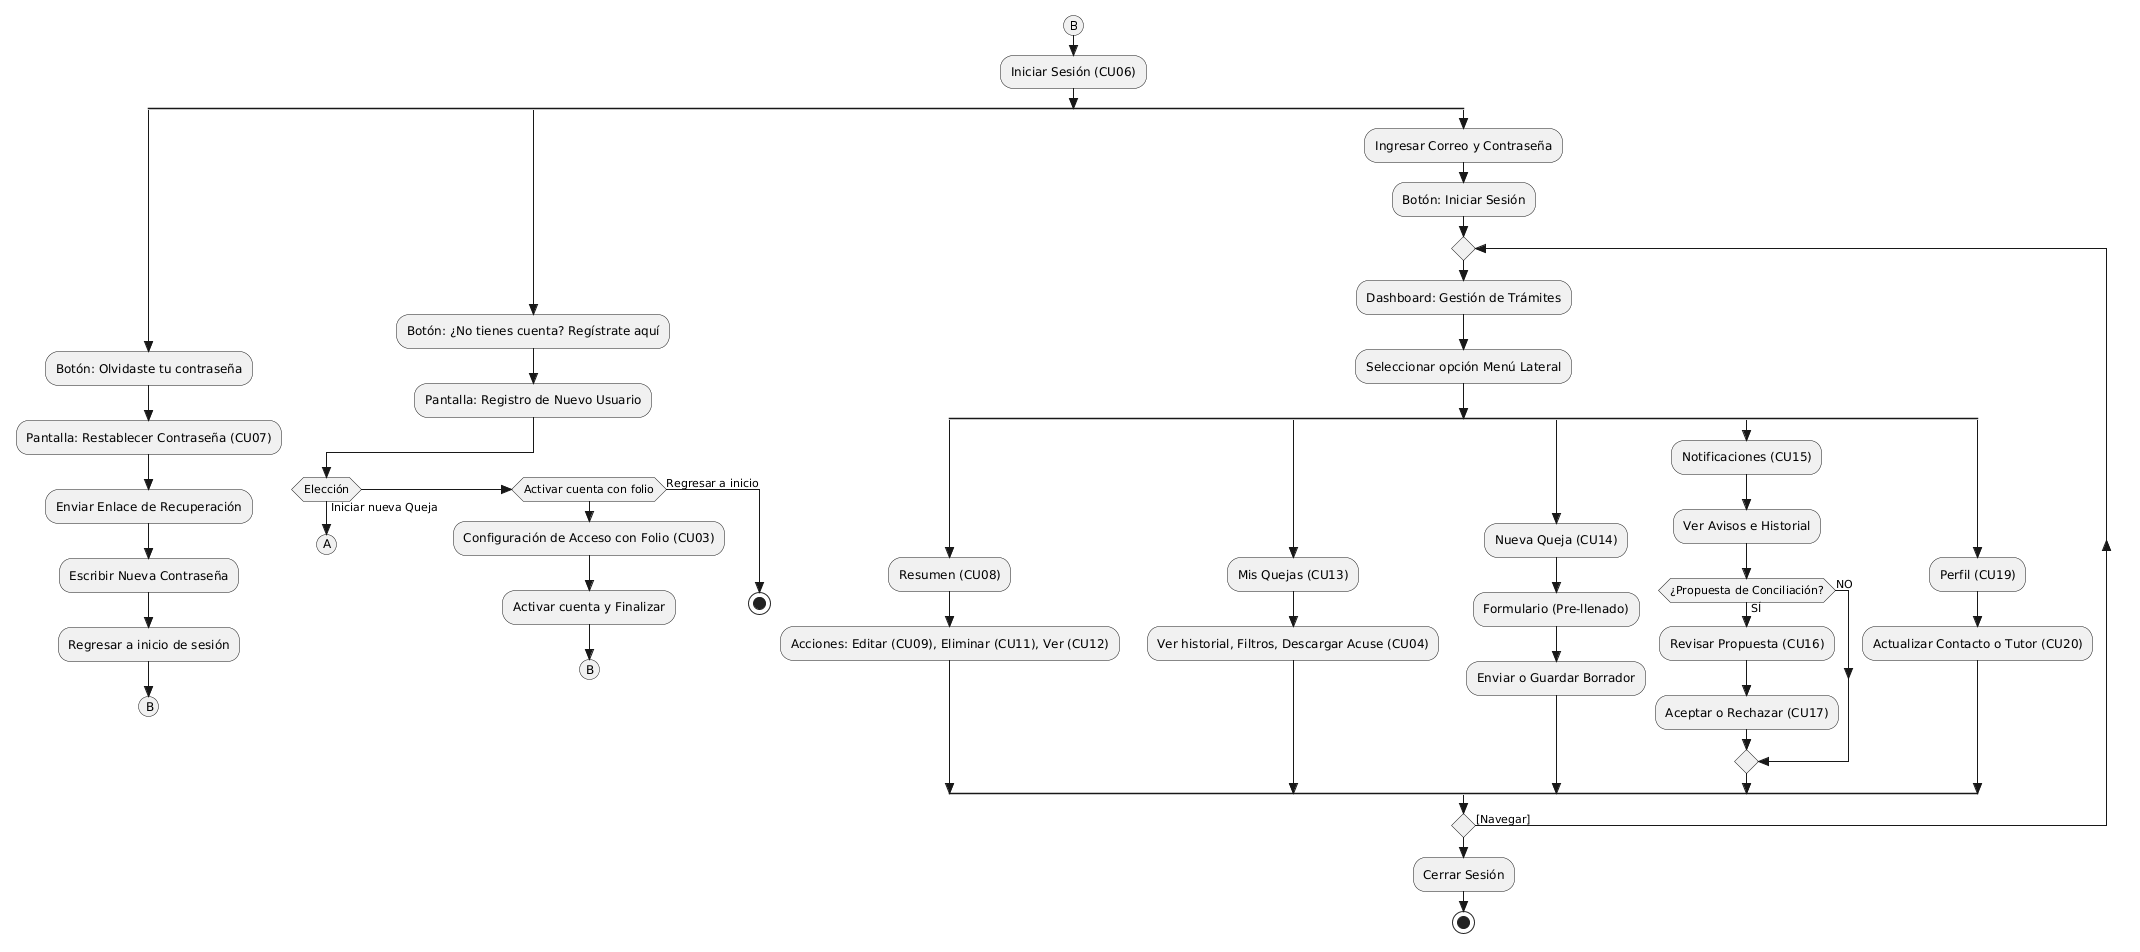
\includegraphics[width=1\textwidth, height=0.90\textheight, keepaspectratio]{imagenes/quejoso/D_Actividad/P2_DA-Quejoso.png}
        \caption{Diagrama de Actividades del Quejoso - Parte 2}
        \label{fig:da_quejoso_parte2}
    \end{figure}

\end{document}
